\chapter{Einleitung}

\section{Aufgabenbeschreibung}

Ziel dieses Semesterprojektes ist es mit Rhapsody, ein mächtiges Tool zur Codegenerierung Design Pattern zu implementieren. Diese werden standardmäßig von Rhapsody nicht angeboten und sollen in Form von Stereotypen während diesem Semester implementiert und getestet werden.
\\
<<<<<<< Updated upstream
In dem vorangegangenen Semester wurde die Umsetzbarkeit der Design Pattern
\begin{itemize}
\item Singleton
\item Observer Pattern
\end{itemize}
belegt. Diese sollen nun dieses Semester vollständig umgesetzt und getestet werden. 
Sind diese Stereotypen dann vollständig in Rhapsody implementiert, ruft Rhapsody 
automatisch Java-Klassen auf, welche dann das als Objektbaum vorliegende Modell 
umbauen können.
\\
Sollte am Ende des Semesters noch genügend Zeit übrig sein, können
selbstverständlich noch weitere Design Pattern umgesetzt werden.

=======
In dem vorangegangenen Semester wurde die Umsetzbarkeit der Design Pattern Singleton und Observer belegt. Weiterhin soll das Design Pattern Guarded Call umgesetzt werden. \\
Diese sollen nun dieses Semester vollständig umgesetzt und getestet werden. Sind diese Stereotypen dann vollständig in Rhapsody implementiert, ruft Rhapsody automatisch Java-Klassen auf, welche dann das als Objektbaum vorliegende Modell umbauen können.

\begin{wrapfigure}[p]
	\centering
	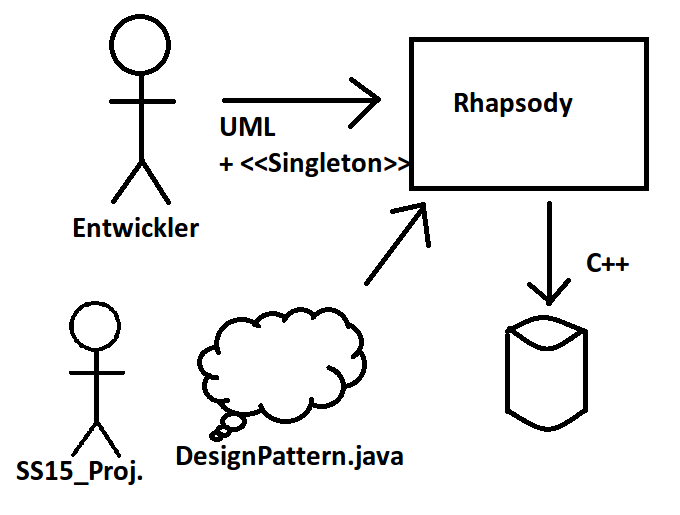
\includegraphics[width=0.66\textwidth]{content/pictures/Simplification}
	\label{pic:bild}
	\caption{blabla}
\end{wrapfigure}

Blabla
>>>>>>> Stashed changes

